\documentclass{article}
\usepackage{tikz}

% Define colors
\definecolor{blueColor}{RGB}{0, 128, 255}
\definecolor{redColor}{RGB}{255, 0, 0}
\definecolor{greenColor}{RGB}{0, 255, 0}

% Define style for nodes
\tikzset{
    mydot/.style={circle, draw=black, fill=white, minimum size=5pt},
    myblue/.style={circle, draw=blueColor, fill=blueColor, minimum size=5pt},
    myred/.style={circle, draw=redColor, fill=redColor, minimum size=5pt},
    myempty/.style={circle, draw=black, fill=white, minimum size=5pt},
    arrow/.style={-stealth, thick, greenColor}
}

\begin{document}

\begin{center}
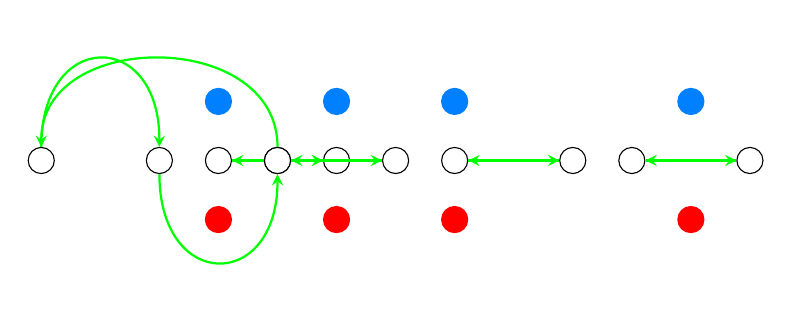
\begin{tikzpicture}[scale=1.5]
    % Draw the first diagram
    \foreach \i in {0, ..., 2} {
        \node[mydot] at (\i, 0) (a\i) {};
    }
    \draw[arrow] (a0) to[out=90, in=90, distance=1cm] (a1);
    \draw[arrow] (a1) to[out=-90, in=-90, distance=1cm] (a2);
    \draw[arrow] (a2) to[out=90, in=90, distance=1cm] (a0);
    
    % Draw the second diagram
    \foreach \i in {0, ..., 1} {
        \node[mydot] at (\i + 1.5, 0) (a\i) {};
    }
    \node[myblue] at (1.5, 0.5) (b0) {};
    \node[myred] at (1.5, -0.5) (b1) {};
    \draw[arrow] (a0) -- (a1);
    \draw[arrow] (a1) -- (a0);
    
    % Draw the third diagram
    \foreach \i in {0, ..., 1} {
        \node[mydot] at (\i + 2, 0) (a\i) {};
    }
    \node[myblue] at (2.5, 0.5) (b0) {};
    \node[myred] at (2.5, -0.5) (b1) {};
    \draw[arrow] (a0) -- (a1);
    \draw[arrow] (a1) -- (a0);
    
    % Draw the fourth diagram
    \foreach \i in {0, ..., 1} {
        \node[myempty] at (\i + 3.5, 0) (a\i) {};
    }
    \node[myblue] at (3.5, 0.5) (b0) {};
    \node[myred] at (3.5, -0.5) (b1) {};
    \draw[arrow] (a0) -- (a1);
    \draw[arrow] (a1) -- (a0);
    
    % Draw the fifth diagram
    \foreach \i in {0, ..., 1} {
        \node[myempty] at (\i + 5, 0) (a\i) {};
    }
    \node[myblue] at (5.5, 0.5) (b0) {};
    \node[myred] at (5.5, -0.5) (b1) {};
    \draw[arrow] (a0) -- (a1);
    \draw[arrow] (a1) -- (a0);
\end{tikzpicture}
\end{center}

\end{document}